\subsection{XmlBuffer}
Protokollen indeholder en buffer klasse, dette var for at tage hensyn til et scenarie hvor en fuld kommando ikke var blevet modtaget og programmet eventuelt terminerede eller lignende. I dette tilfælde ville programmet ved næste opstart kunne modtage resterende del af kommandoen. Dette betyder at der fra Protocol klassen indimellem kaldes på bufferen for at se om der er nogle indkomne kommandoer og hvis dette er tilfældet, så håndteres disse, og på den mådes undgås fejl med ukomplette beskeder.

Der blev derudover oprettet et interface, IProtocolBuffer, dette var i tilfælde af at systemet senere skulle udvides med flere buffere, så systemet ville kunne kommunikere med flere/andre kodesprog.

\begin{figure}[H]
	\centering
	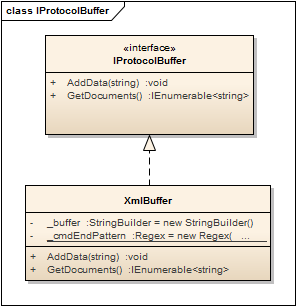
\includegraphics[width=0.4\textwidth]{Systemdesign/SharedLib/Images/Klasser/IProtocolBuffer.png}
	\caption{XmlBuffer der implementerer IProtocolBuffer}
	\label{fig:klasseXmlBuf}
\end{figure}
